\chapter{CLI Technicalities}\label{appendix:cli}

We carefully considered what libraries to use for this CLI to be flexible and easily extendible.
The OAK CLI initially used Python's argparse \cite{python_argparse} and argcomplete \cite{python_argcomplete}.
Argparse is an established feature-rich standard library.
Its downside is that it requires a lot of boilerplate code, especially when the argument structure is a complex nested hierarchy.
Argcomplete enables auto-/tab-completions of CLI commands.
Enabling this functionality in a pure Python tool can be tricky and require specific workarounds.
OAK CLI now uses Typer \cite{typer}.
Typer requires minimal decorator augmentations to enable CLI applications.
This is possible because Typer smartly utilizes available Python-type hints in function signatures.
It automatically comes with auto/tab completion and includes highly readable, pretty UI features powered by Rich \cite{rich}.
Rich is a prominent library for Python terminal formatting.
Typer is built on top of Click \cite{click}, one of the most popular Python CLI frameworks.
The downside of Typer is that it is still in relatively early development.
It lacks a first major release version.
It has some minor cutbacks compared to argparse, but discussing those would bloat this work.

\subsection{CLI Commands}

The root command is \texttt{oak}.
The following is a simplified overview that does not depict or explain every available option and feature to avoid bloating this work because the CLI underlies active change.
Most of the subcommands below have shorter aliases to help accelerate typing.
\vspace{5mm}
\newline
\textbf{Auxiliary/Meta}
\begin{itemize}
    \item [\texttt{help}]:
        Shows auxiliary information.
        This flag is available for every subcommand.
    \item [\texttt{version}]:
        Shows the version of the currently installed OAK CLI.
    \item [\texttt{api-docs}]:
        Shows a link to Oakestra's Swagger API documentation page.
\end{itemize}
\vspace{5mm}
\textbf{Applications}
\begin{itemize}
    \item [\texttt{a}]:
        The pre-command to work with Oakestra applications.
        \begin{itemize}
            \item [\texttt{create}]:
                Creates one or multiple Oakestra applications based on the provided SLA.
                The additional optional flag \texttt{-d} automatically deploys all services present in the application SLA.
                The CLI comes with pre-build common app SLAs that users can inspect and modify to their liking.
            \item [\texttt{delete}]:
                Deletes one or all applications.
            \item [\texttt{show}]:
            Displays an overview of the current applications.
            The overview comes in three different variations.
            The simple view shows a table of all applications with minimal additional information, such as their number of services and ID.
            The detailed view shows a table with additional information columns.
            The exhaustive view shows the verbatim underlying JSON object showing all available details.
            The \texttt{-v} flag (verbosity) toggles between these versions.
            This overview gets printed a single time.
            The \texttt{-l} flag (live-display) starts an overview that refreshes itself every three seconds.
        \end{itemize}
\end{itemize}
\vspace{5mm}
\textbf{Services}
\begin{itemize}
    \item [\texttt{s}]:
        The pre-command to work with Oakestra services.
        Remember that services are part of applications.
        They cannot be created in isolation.
        Usually, one creates an application and then deploys the services mentioned in its SLA.
        \begin{itemize}
            \item [\texttt{deploy}]:
                Deploys a new service instance.
            \item [\texttt{undeploy}]:
                Un-deploys a specific or all service instances of a single or every service.
            \item [\texttt{show}]:
                The show subcommand for services works exactly as for applications, including the verbosity and live-display flags.
                The difference between them is the displayed information.
            \item [\texttt{inspect}]:
                The inspect command shows detailed information of a single service instead of all services.
                The main benefit of inspecting a service is to see its latest logs.
                This command also offers the \texttt{-l} (live-display) flag, so users can observe service instance logs close to real-time.
        \end{itemize}
\end{itemize}
\vspace{5mm}
\textbf{FLOps}
\begin{itemize}
    \item [\texttt{addon flops}]:
        FLOps is one of Oakestra's addons.
        The \texttt{addon} subcommand tells the CLI to show addon-related commands.
        The \texttt{flops} subcommand shows the available FLOps CLI commands.
        \begin{itemize}
            \item [\texttt{project}]:
                Starts a new FLOps project.
                The CLI currently provides several pre-build project SLAs.
                They use different ML frameworks such as Scikit-learn or Pytorch with different datasets such as MNIST or CIFAR-10.
                They use varying training configurations, including various numbers of learners and training rounds.
                SLAs are available for classic and HFL projects.
            \item [\texttt{tracking}]:
                This command returns the URL to the user's tracking server.
                If no tracking server exists, it will create one.
            \item [\texttt{mock-data}]:
                Launches a mock data provider based on the specified FLOps Helper SLA.
            \item [\texttt{clear-registry}]:
                Clears the image registry hosted via the FLOps management.
            \item [\texttt{reset-database}]:
                Resets the FLOps management database.
            \item [\texttt{restart-management}]:
                Restarts all FLOps management components.
        \end{itemize}
\end{itemize}
\vspace{5mm}
\textbf{Oakestra Docker Containers}
\begin{itemize}
    \item [\texttt{d}]:
        Oakestra's control plane runs on two Docker compose files for the root and cluster aggregators.
        When developing and modifying the code of one of these components, many developers rebuilt and restarted the entire compose file or even the entire cluster to see the changes take effect.
        This command allows one to rebuild a single container of an Oakestra compose file directly, which leads to the same result.
        Rebuilding a single container takes a fraction of the time required to rebuild the entire compose file or cluster.
        Thus, this command enables accelerated development/change cycles.
        Users can decide if they want to restart or rebuild an Oakestra container.
        A \texttt{--cache-less} flag is available for the rebuild command to ensure all changes are propagated.
\end{itemize}
\vspace{5mm}
\textbf{Worker Node}\newline
The w pre-command includes commands that are specific for worker nodes.
\begin{itemize}
    \item [\texttt{ctr delete-images}]:
        This command is especially useful when developing images.
        For example, a worker node must pull the FLOps image builder service image before running its container.
        When developing this image and pushing it as the same (latest) version, containerd sees that the tag is already present locally and does not pull the updated version.
        After using this command, one can be sure that the next image used will be the latest pushed one.
\end{itemize}
\vspace{5mm}
\textbf{Installer}\newline
The \texttt{installer} pre-command hosts commands to install and set up necessary dependencies on the host machine.
The OAK-CLI uses Ansible to perform the installation.
\begin{itemize}
    \item [\texttt{fundamentals}]:
        The fundamentals command will install core dependencies such as Git, Docker, and Golang.
\end{itemize}
\vspace{5mm}
\textbf{Configuration}\newline
The CLI is configurable to avoid overwhelming users with all these available features and only shows applicable and useful commands for their concrete use case.
It stores these configurations persistently in a config file via Python's configparser library.
Users should set their intended use case via the CLI to unlock the relevant commands.
As a result, the CLI can be a fine-tuned tool for different user groups and scenarios.
\begin{itemize}
    \item [\texttt{c}]:
        The pre-command to enter the CLI configuration commands.
        \begin{itemize}
            \item [\texttt{show-config}]:
                Displays the current CLI configuration.
            \item [\texttt{local-machine-purpose}]:
                This command allows users to pick their preferred CLI features.
            \item [\texttt{key-vars}]:
                Various commands depend on properly configured CLI key variables.
                If users try to run a command where a key variable is undefined, the CLI will ask the user to define it first.
                One example of such a key variable is the path to the cloned Oakestra or FLOps repository.
                These pointers let the CLI know where Oakestra's or FLOps' compose files reside.
        \end{itemize}
\end{itemize}
\vspace{5mm}
\textbf{Evaluation}\newline
The evaluation commands are very experimental and might get removed from the CLI.
We used them to run the evaluations for FLOps.

\begin{itemize}
    \item [\texttt{evaluate}]:
        Shows a list of commands to control evaluations.
        This includes starting manual or automatic evaluation cycles or displaying CSV files that get populated during evaluation.
        Further details are available in the evaluation chapter.
\end{itemize}

\subsection{CLI Showcase}

This subsection presents several screenshots of the current OAK CLI.
It only focuses on visually interesting command outputs. 
The CLI is in active development and is subject to change.
The first screenshot \ref{fig:cli_main_help} shows the main help text of the OAK CLI.
Figure \ref{fig:cli_app_views} depicts an example of a single app displayed in different verbosity modes.
Figure \ref{fig:cli_service_views} shows the simple and detailed view of the services from the single app from the previous figure.
We ommit showing the exhaustive view because its JSON representation is very verbose.
Screenshot \ref{fig:cli_service_inspection} shows the detailed inspection view of a concrete service with two instances.
The grey text at the top shows service properties.
The light blue text underneath it presents service instance information.
The green text shows the latest logs of each deployed instance.

\begin{figure}[p]
    \begin{adjustwidth}{-0.1\paperwidth}{-0.1\paperwidth}
        \centering
        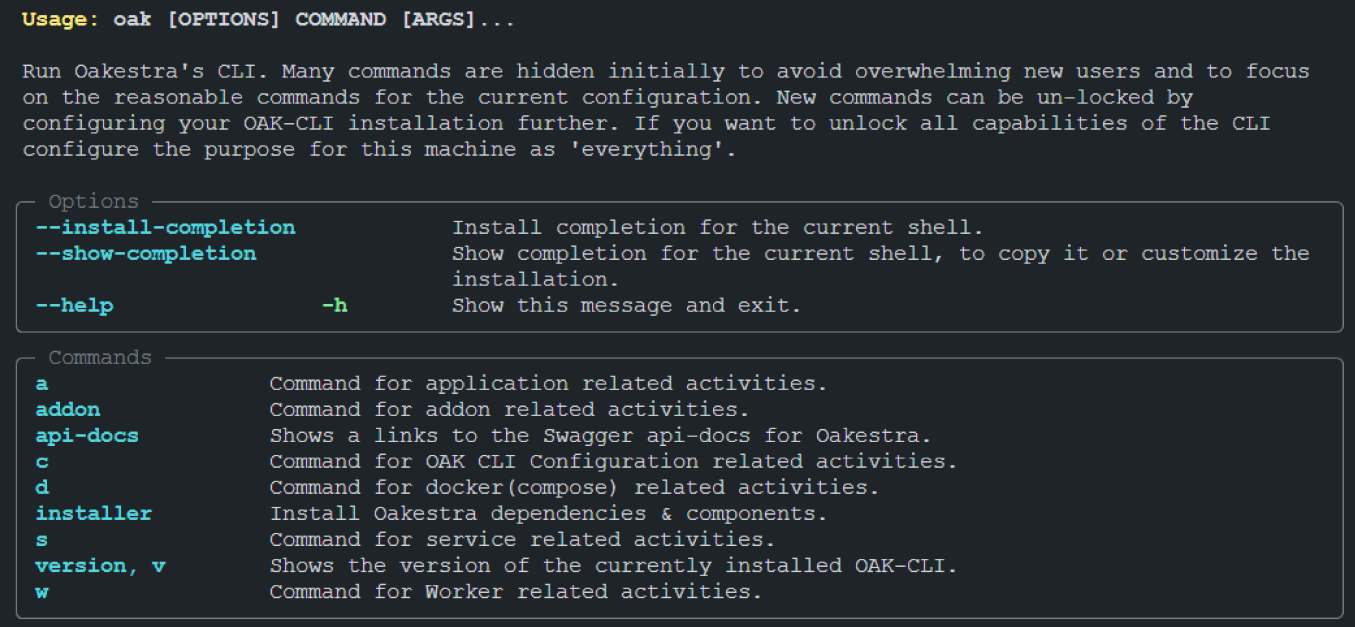
\includegraphics[width=0.90\paperwidth]{cli_main_help.png}
        \caption{OAK CLI main help text: oak -h}
        \label{fig:cli_main_help}
    \end{adjustwidth}

    \begin{adjustwidth}{-0.2\paperwidth}{-0.2\paperwidth}
        \centering
        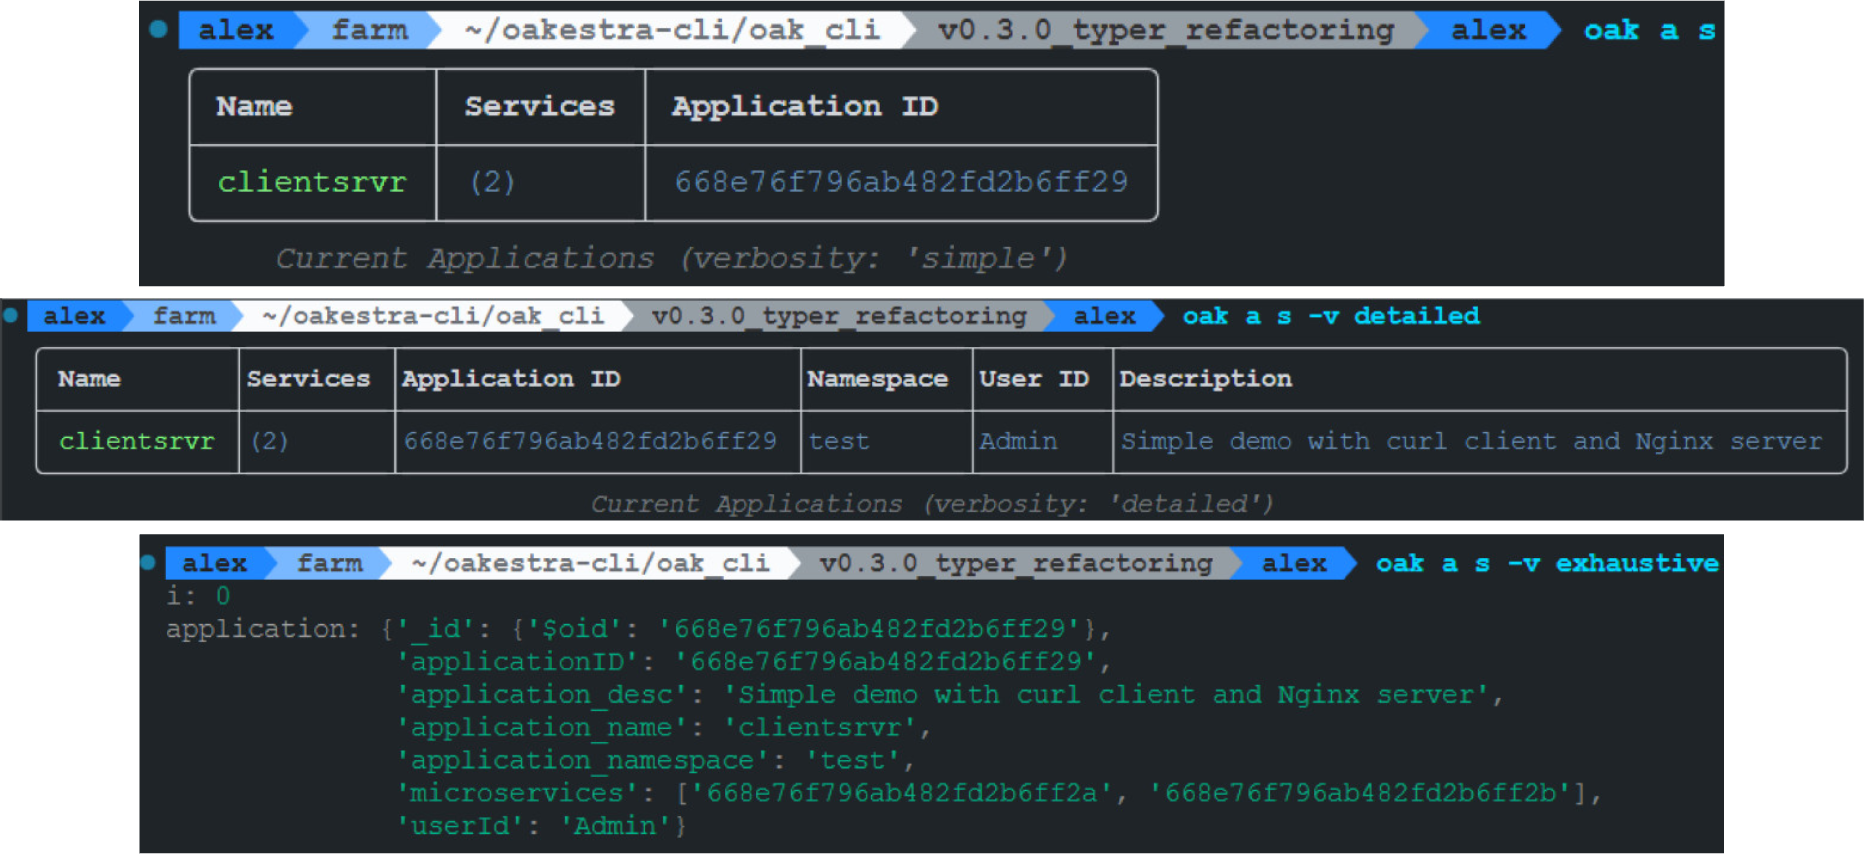
\includegraphics[width=0.95\paperwidth]{cli_app_verbosities.png}
        \caption{OAK CLI Application Views}
        \label{fig:cli_app_views}
    \end{adjustwidth}
\end{figure}

\begin{figure}[p]
    \centering
    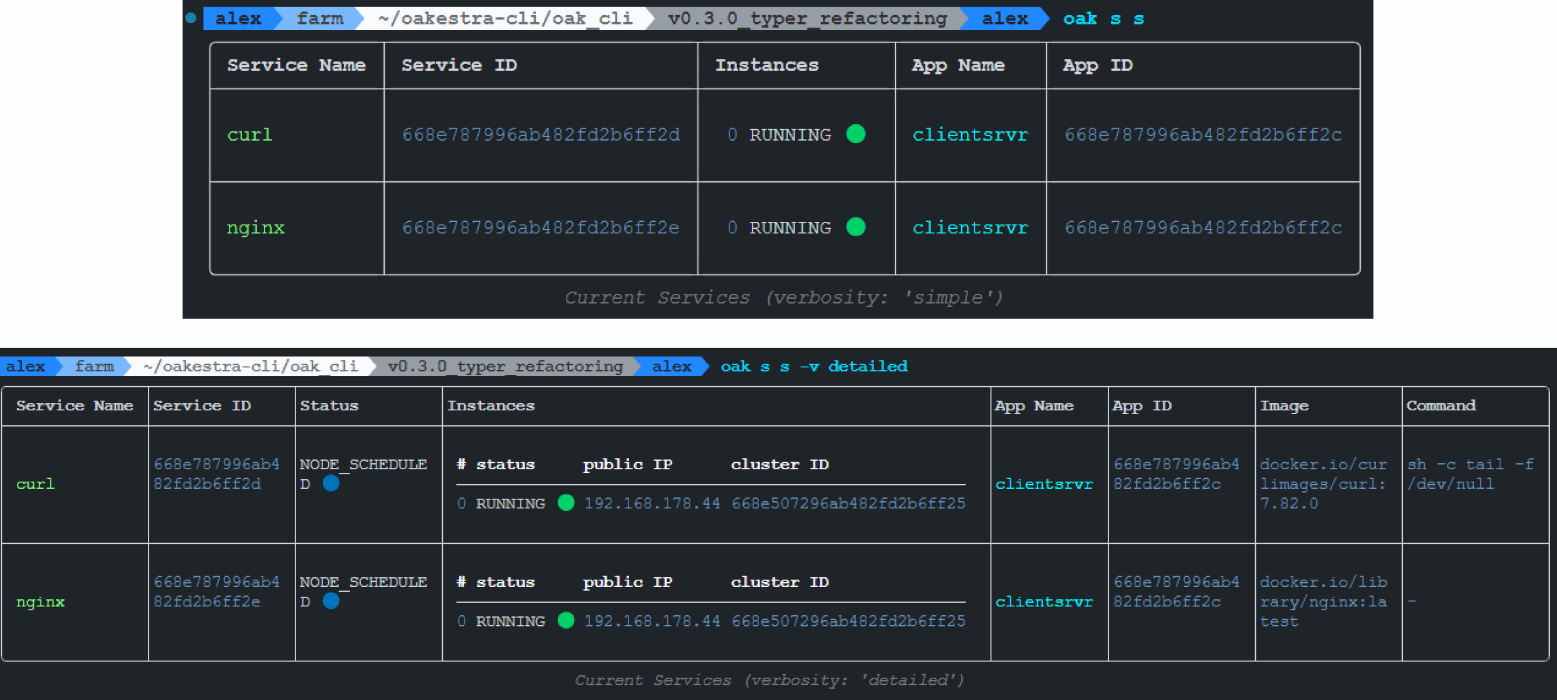
\includegraphics[angle=90,origin=c,height=0.74\textheight]{cli_services_verbosities.png}
    \caption{OAK CLI Service Views}
    \label{fig:cli_service_views}
\end{figure}

\begin{figure}[p]
    \begin{adjustwidth}{-0.1\paperwidth}{-0.1\paperwidth}
        \centering
        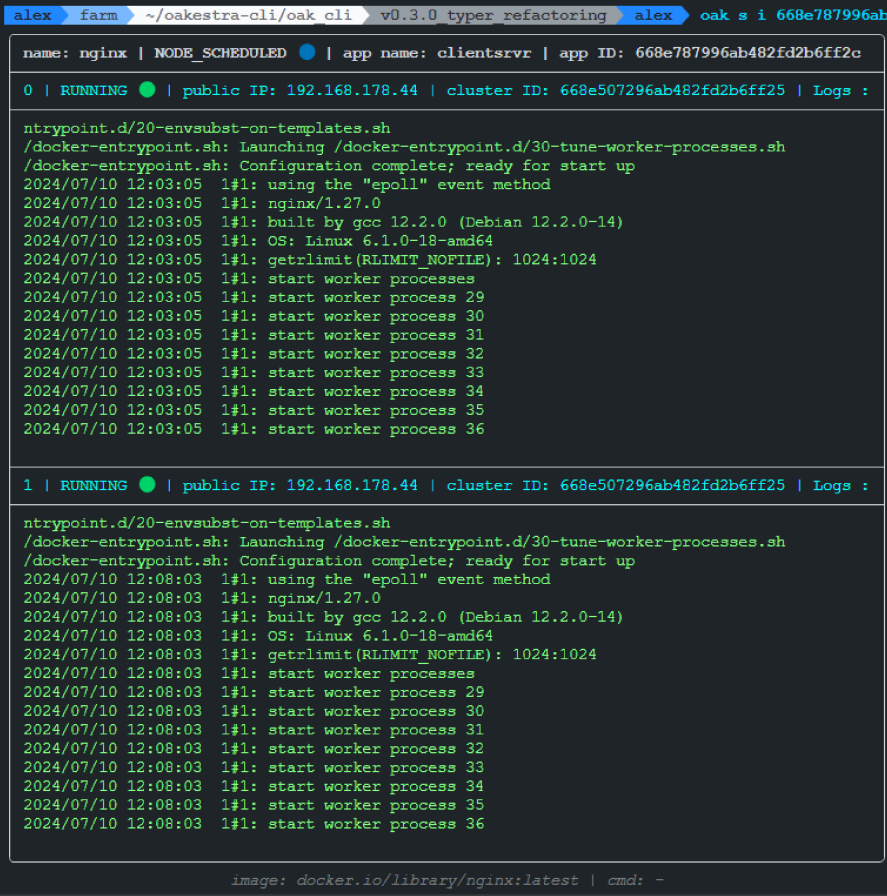
\includegraphics[width=0.80\paperwidth]{cli_service_inspect}
        \caption{OAK CLI Service Inspection}
        \label{fig:cli_service_inspection}
    \end{adjustwidth}
\end{figure}
